\chapter{Specifikace}\label{chapter:specifikace}

% strana 6 a 9
Sommerville~\cite{sommerville_softwareengineering_2011} uvádí fundamentální aktivity softwarového inženýrství: specifikace, vývoj, validace a evoluce.
Dále definuje softwarovou specifikaci jako aktivitu, při které zákazníci a inženýři definují software, který má být vyprodukován, a omezení na jeho provoz.

V této kapitole definujeme software, který budeme tvořit, pomocí požadavků uživatele, případů užití, konceptuálního schématu a procesů.

\section{Požadavky}

Požadavky na softwarový systém jsou popisy toho, co by měl systém dělat -- služby, které poskytuje, a omezení na jeho provoz.
Tyto požadavky by měly reflektovat potřeby zákazníka na systém a jeho účel, uvádí Sommerville~\cite[s.~83]{sommerville_softwareengineering_2011}.

Požadavky na funkce systému nazýváme funkční.
Požadavky na provoz systému a jeho omezení nazýváme nefunkční.

Dále uvedeme vybrané funkční a nefunkční požadavky z pohledu uživatele systému.

\subsection{Funkční požadavky}
\newlist{enumfp}{enumerate}{1}
\setlist[enumfp]{label=\textbf{FP\hyp{}\arabic*},ref=FP\hyp{}\arabic*}

\subsubsection*{Projekt}
\begin{enumfp}
  \item V systému bude možné vytvořit nový projekt.
  \item Projekt bude možné uložit.
  \item Projekt bude možné načíst.
  \item Projekt bude možné pojmenovat pro odlišení od ostatních projektů.
  \item Jednotlivé diagramy bude možné exportovat do rastrového i vektorového formátu.
  \item Do těchto exportovaných formátů bude volitelně možné vložit projekt, který z nich pak bude možné načíst.
  Tímto bude projekt možné otevřít jak v prohlížeči obrázků (a zobrazit rastrově nebo vektorově diagram), tak v našem systému a pokračovat v práci.
\end{enumfp}

\subsubsection*{Diagramy}
\begin{enumfp}[resume]
  \item Zobrazení každého diagramu bude možné posouvat myší.
  \item Zobrazení každého diagramu bude možné přibližovat a oddalovat kolečkem myši.
  \item Posunutí a přiblížení bude volitelně možné synchronizovat mezi všemi diagramy.
  \item Systém bude kontrolovat validitu uživatelem vytvořených konstruktů.
  \item Elementy bude možné posunovat držením levého tlačítka myši a tažením.
  \item Související elementy napříč diagramy se budou posouvat společně.
  \item Vlastnosti všech objektů bude možné měnit (popisky, typ, pozice).
  Tyto změny budou reflektovány v ostatních diagramech.
  \item Při držení klávesy \keys{\ctrl} bude možné zvolit více objektů najednou postupným klikáním levého tlačítka myši.
  \item Veškeré elementy bude možné z diagramu mazat alespoň klávesou \keys{Delete}.
  \item Všechny elementy bude možné zvolit levým tlačítkem myši.
\end{enumfp}

\subsubsection*{ER Diagram}
\begin{enumfp}[resume]
  \item Do diagramu bude možné přidat entitní typ.
  \item Do diagramu bude možné přidat vztahový typ.
  \item Do diagramu bude možné přidat atribut.
  \item Mezi jednotlivými elementy diagramu bude možné přidat spojovací čáru.
  \item U spojení bude možné specifikovat a zobrazit kardinalitu.
  Dolní mez bude buď 0 nebo 1, horní mez 1 nebo $n$.
  Výchozí kardinality ($1..1$) nebudou zobrazeny.
  \item Bude možné vytvořit ISA hierarchii mezi entitními typy.
  \item Uživatel bude moct využít předpřipravené konstrukty, které bude možné vložit do diagramu.
  Například se může jednat o ISA hierarchie s předpřipravenými entitami.
\end{enumfp}

\subsubsection*{Schématická kategorie}
\begin{enumfp}[resume]
  \item Objekty a morfismy schematické kategorie bude možné přidávat a mazat, přičemž tato změna se odrazí v ostatních diagramech.
  \item V diagramu se zobrazí data o objektech a morfismech včetně kardinalit a popisků.
  Výchozí kardinality ($1..1$) se zobrazovat nebudou.
  \item Při zvolení objektu se zvýrazní všechny objekty v okolí, které ho identifikují (např. barevně, vzdálené identifikátory jinou barvou).
\end{enumfp}

\subsubsection*{Vizualizace schematické kategorie}
\begin{enumfp}[resume]
  \item Vizualizace schematické kategorie ze schematické kategorie vytěží sémantiku a vizualizuje ji různými tvary.
  \item Při zvolení objektu se barevně zvýrazní bezprostřední a vzdálené identifikátory různými barvami.
\end{enumfp}

\subsection{Nefunkční požadavky}
\newlist{enumnfp}{enumerate}{1}
\setlist[enumnfp]{label=\textbf{NFP\hyp{}\arabic*},ref=NFP\hyp{}\arabic*}

\begin{enumnfp}
  \item Aplikaci bude možné používat na všech běžných desktopových operačních systémech.\label{nfp:can-use-everywhere}
  \item Nesmí dojít ke ztrátě práce při náhlém ukončení aplikace kvůli interním či externím vlivům.
  To může být zařízeno např. průběžným ukládáním práce.
  \item Aplikaci bude možné používat i při výpadku internetového připojení.
  \item V rámci bezpečnosti žádná data týkající se práce na projektu neopustí zařízení klienta, pokud tak klient explicitně neučiní (například export a přesun souboru).\label{nfp:safety}
  \item Aplikace bude navržena tak, aby bylo možné bez větších komplikací rozšířit její funkcionalitu (např. přidat podporu UML).
  \item Aplikace bude nenáročná na provoz a investice provozovatele.\label{nfp:nenarocnost}
\end{enumnfp}

\section{Entity}\label{section:conceptual-model}

V této kapitole představíme konceptuální model aplikace.
Jedná se o část světa, na kterou vymezujeme svůj diskurz.
Využijeme k tomu prostředky \acrfull{uml}~\cite{omg_uml_2017}.

\begin{figure}[!htb]
  \centering
  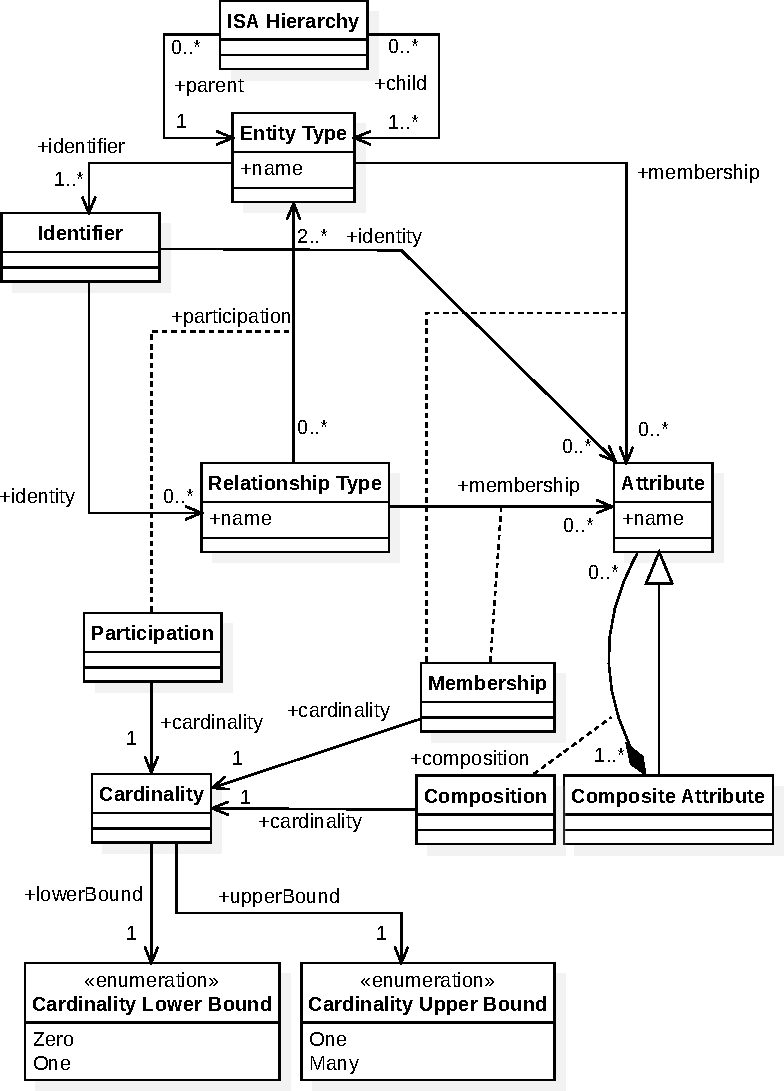
\includegraphics[width=\maxwidth{\textwidth}]{../img/diagrams/er-diagram-model.pdf}
  \caption{Konceptuální schéma -- ER diagram}
  \label{fig:class-diagram:er-diagram}
\end{figure}

Na Obrázku~\ref{fig:class-diagram:er-diagram} je \acrshort{UML} konceptuální schéma modelující \acrshort{er} diagram.
Obsahuje třídy odpovídající všem konstruktům popsaných v Sekci~\ref{section:entity-relationship} -- entitní typ, vztahový typ, atribut, složený atribut, ISA hierarchie, kardinalita a identifikátor.
Entitní typ, vztahový typ i atribut mají složku vyjadřující jejich uživatelské jméno.
Navíc jsme uvedli tři třídy asociace k asociacím mezi těmito objekty, které mají všechny svou kardinalitu:
\begin{itemize}
  \item \emph{Membership} (členství) vyjadřuje vztah mezi entitním typem nebo vztahovým typem a atributem.
        Toto jméno vyjadřuje, že atributy považujeme za členy (members) entitních a vztahových typů.
        Entitní i vztahové typy mají buď žádný atribut, nebo libovolné množství atributů.
  \item \emph{Composition} (složení) vyjadřuje vztah mezi složeným atributem a atributy, z kterých se skládá.
        Složený atribut musí mít alespoň jeden atribut, jinak ho nepovažujeme za složený.
  \item \emph{Participation} (účast) vyjadřuje vztah mezi vztahovým typem a entitními typy, které se daného vztahového typu účastní.
\end{itemize}

Názvy pro naše tři třídy asociace byly inspirovány \acrshort{er} diagramem, který modeluje \acrshort{er} od Atzeniho~\cite[Obr.~5.22]{atzeni_database_1999}

Tyto tři třídy asociace jsme mohli sjednotit do jedné, protože všechny obsahují pouze jednu instanci kardinality.
Tím by však zanikl jejich rozlišný význam, který může být v určitém kontextu důležitý.
Mohli bychom jim také uvést společného předka, ale to považujeme za zbytečné a konceptuálně nemnoho vypovídající.

Kardinalita se skládá ze dvou složek, jejichž možné hodnoty jsou dány enumeracemi.
To vyjadřuje naše omezení, která jsme na kardinalitu položili.

ISA hierarchie se přesně podle definice skládá z jednoho entitního typu rodiče a jednoho či více entitních typů dětí.
Mohli jsme místo toho modelovat vztah jednoho rodiče s jedním dítětem, ale v \acrshort{er} je důležité nad těmito vztahy uvažovat po $n$-ticích.

Identifikátory jsme namodelovali bez rozlišení významu externích a interních identifikátorů, protože to je vlastnost, která pro každý identifikátor vyplyne až v instanci modelu.
Každý entitní typ musí mít z definice našeho \acrshort{er} modelu alespoň jeden identifikátor (nebo více).
Ten se může skládat z libovolného množství atributů a vztahových typů.
V instanci modelu bychom označili identifikátor mající alespoň jeden vztahový typ jako externí, jinak interní.
Přestože model technicky povoluje i identifikátory bez členů, nejsou takové identifikátory validní.

\begin{figure}[!htb]
  \centering
  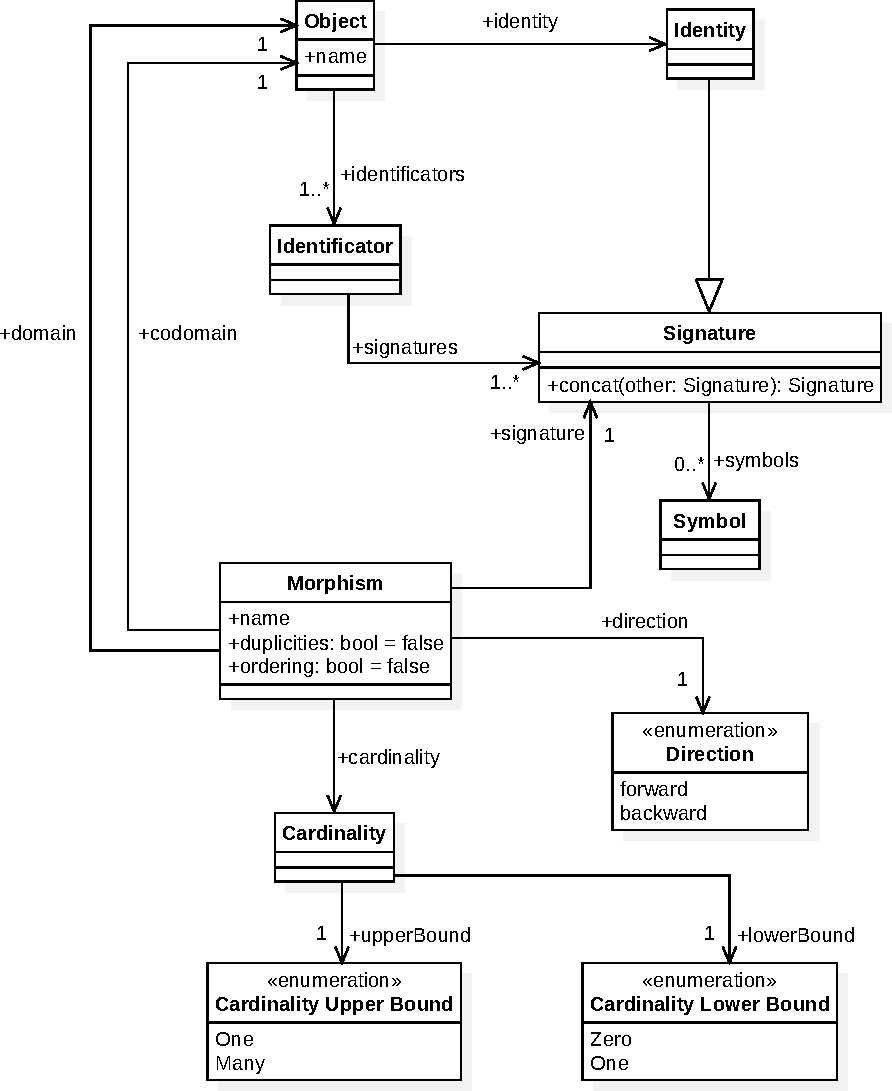
\includegraphics[width=\maxwidth{\textwidth}]{../img/diagrams/schema-category-model.pdf}
  \caption{Konceptuální schéma -- schematická kategorie}
  \label{fig:class-diagram:schemcat}
\end{figure}

Na Obrázku~\ref{fig:class-diagram:schemcat} je konceptuální model schematické kategorie.
Stěžejními třídami v modelu jsou objekt, morfismus a signatura.

Signatura se skládá z jednotlivých symbolů, kterých může být 0 (prázdný řetězec $\varepsilon$) a více.
Jedná se totiž z Definice~\ref{def:signature} o řetězec.
Jednotlivými symboly může být úplně cokoli, dle volby abecedy.
Podle volby v implementaci může jít o znaky, řetězce, či libovolné objekty.
Signatury lze řetězit za sebe, což jsme vyjádřili operací \texttt{concat}\footnote{z anglického \emph{to concatenate} -- zřetězit, spojit},
která vrátí novou signaturu vzniklou zřetězením této a jiné, předané parametrem \texttt{other}.
Pokud označíme danou instanci signatury \texttt{tato}, zřetězení by mělo probíhat v pořadí \texttt{tato} $\cdot$ \texttt{other}, stejně jako je to běžné u jazyků.
Až v implementaci by se mělo dbát na správné pořadí při skládání morfismů, které je opačné.

V konceptuálním modelu vyjadřujeme, že každý objekt musí mít alespoň jeden identifikátor, který se skládá ze signatur.
Speciálně tímto identifikátorem může být i $\set{\set{\varepsilon}}$, protože signatura může být prázdný řetězec.
Jak jednotlivé identifikátory, tak celá jejich sada u daného objektu, by měla být množina, a proto se nemusí dbát na pořadí a duplicity.

Pro morfismy je vyjádřeno, že by měl mít každý svou signaturu.
Mohli bychom morfismy vydělit na námi definované druhy specializováním třídy morfismu na bázový, odvozený a identitní.
U bázových by bylo vyjádřeno, že jejich signaturou je pouze jediný symbol.
U odvozených je jejich signaturou již namodelovaná třída signatury.
A u identitních je jejich signaturou prázdný řetězec, tedy konstanta.
Toto rozdělení nám však pro konceptuální model přijde zbytečné, protože se jedná o vlastnost morfismu, která vyplyne z toho, z kolika symbolů se jeho signatura skládá.

Další prvky konceptuálního modelu schematické kategorie jsou zřejmé a vycházejí přímo z definice schematické kategorie ze Sekce~\ref{section:schemcat}.

\begin{figure}[!htb]
  \centering
  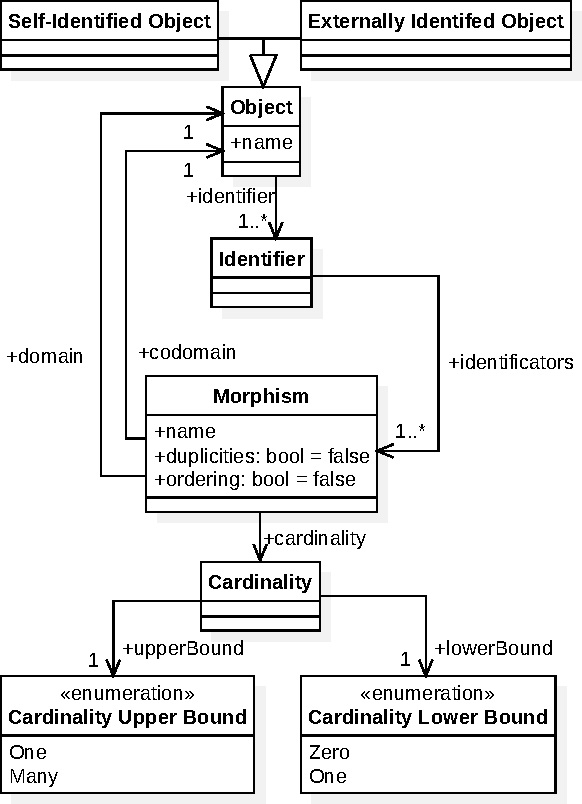
\includegraphics[width=\maxwidth{\textwidth}]{../img/diagrams/scv-model.pdf}
  \caption{Konceptuální schéma -- \acrlong{vsk}}
  \label{fig:class-diagram:scv}
\end{figure}

Konceptuální model \acrfull{vsk}, který je na Obrázku~\ref{fig:class-diagram:scv}, je podobný konceptuálnímu modelu schematické kategorie, s několika málo rozdíly.
Koncept signatury ve vizualizaci zaniká.
Místo toho jsou identifikátory objektů tvořeny přímo navazujícími morfismy.
Objekty a morfismy ztrácí svoji identitu, resp. signaturu.
Ta konceptuálně ve \acrshort{vsk} není.

V konceptuálním modelu \acrshort{vsk} nově rozlišujeme dva typy objektů -- self-identifikovaný objekt (definovaný v Sekci~\ref{section:vsk}) a naproti tomu externě identifikovaný objekt.
Rozlišujeme je kvůli tomu, že ve \acrshort{vsk} jsou zobrazeny různými tvary.

Protože ve \acrshort{vsk} zanikají inverzní morfismy, mizí z konceptuálního modelu v morfismu i složka udávající směr.

Doména a kodoména nejsou ve \acrshort{vsk} konceptem a mohli bychom je pojmenovat např. zdrojový a cílový objekt.
Nicméně pro přehlednost a snahu o menší komplikaci konceptuálních rozdílů ponecháme i ve \acrshort{vsk} názvy doména a kodoména.

Další koncepty jsou totožné konceptuálním modelem schematické kategorie.

\section{Procesy}

Součástí specifikace softwarového systému jsou i procesy.
Každý proces popisuje konceptuální kroky, které vedou k dosažení nějakého cílového stavu.
Tyto kroky jsou definovány pouze na konceptuální úrovni, takže bez vtahu např.~k plánovanému uživatelskému rozhraní.

Požadavky popsaly, co systém má umět.
Procesy je rozšíří o to, jakým způsobem toho aktéři mohou dosáhnout a jaké kroky k výslednému stavu vedou.

\subsubsection*{Modelování entitního typu v \acrshort{er} diagramu}

Uživatel mezi existující elementy diagramu vloží nový entitní typ.
Tento entitní typ bude chtít pojmenovat.
K entitnímu typu bude uživatel potřebovat přidat atributy.
Dále bude entitní typy potřebovat přidat do vztahů, tedy spojit s existujícími vztahovými typy.

Entitní typ bude moci změnit na jiný druh elementu v \acrshort{er} diagramu (atribut, vztahový typ).

Kroky zahrnují:
\begin{enumerate}
  \item Přidání nového prvku do diagramu.
  \item Zvolení druhu prvku -- entitní typ.
  \item Zadání popisku (názvu entitního typu).
  \item Zvolení pozice entitního typu v diagramu.
  \item Případné přidání atributů k entitnímu typu a volba jejich kardinality.
  \item Přidání entitního typu do ISA hierarchie s jinými entitními typy.
  \item Zvolení jednoho a více identifikátorů entitního typu.
        Toto není třeba pokud byl entitní typ přidán do hierarchie, pak dědí identifikátory.
  \item Případně přidání daného entitního typu jako účastníka libovolného počtu existujících vztahových typů.
\end{enumerate}

\subsubsection*{Modelování vztahového typu v \acrshort{er} diagramu}
Uživatel bude dále chtít do \acrshort{er} diagramu přidat vztahový typ.
Vztahový typ musí mít alespoň dva (ne nutně různé) účastníky, jimiž mohou být pouze entitní typy.

Kroky zahrnují:
\begin{enumerate}
  \item Přidání nového prvku do diagramu.
  \item Zvolení druhu prvku -- vztahový typ.
  \item Zadání popisku (názvu vztahového typu).
  \item Zvolení pozice vztahového typu v diagramu.
  \item Zvolení účastníků vztahového typu.
  \item Zvolení kardinalit účastníků vztahového typu.
\end{enumerate}

\subsubsection*{Mazání prvků v \acrshort{er} diagramu}

Při modelování může uživatel přehodnotit model a odstranit některé prvky, načež je případně nahradit jinými.

Kroky zahrnují:
\begin{enumerate}
  \item Zvolení prvku či prvků v diagramu, které chceme smazat.
  \item Odstranění prvků z diagramu.
  \item Odstranění souvisejících spojení s jinými prvky diagramu.
  \item U entitních typů odstranění případných identifikátorů z diagramu.
\end{enumerate}

\subsubsection*{Volba identifikátoru entitního typu v \acrshort{er} diagramu}

Při modelování entitního typu bude uživatel chtít přidat jeho identifikátory.

Kroky zahrnují:
\begin{enumerate}
  \item Zvolení jednoho a více atributů či vztahových typů, které mají tvořit nový identifikátor.
  \item Pokud je ve vztahovém typu zúčastněn entitní typ víckrát, je nutné zvolit spojení, které má být identifikátorem.
  \item Kontrola neexistence redundantních identifikátorů, které byly popsány v Sekci~\ref{section:entity-relationship}.
  \item Validace neexistence cyklů slabých entitních typů a hierarchií, jak byla popsána v Sekci~\ref{section:entity-relationship}.
\end{enumerate}

\subsubsection*{Změna typu elementu \acrshort{er} diagramu}

Uživatel potřebuje měnit typ elementu diagramu, například když se rozhodne, že je v daném případě lepší modelovat entitní typ jako složený atribut.

Kroky zahrnují:
\begin{enumerate}
  \item Specifikace elementu diagramu, který bude uživatel měnit (entitní typ, vztahový typ, nebo atribut).
  \item Volba typu elementu, na který se má element změnit.
  \item Kontrola validity diagramu. Úpravou mohl vzniknout nevalidní \acrshort{er} diagram.
\end{enumerate}

\subsubsection*{Přesun a změna přiblížení plátna}

Při modelování se uživatel bude chtít zaměřit na jednu část diagramu přesunem plátna a přiblížením.

Kroky zahrnují
\begin{enumerate}
  \item Zvolit diagram, jehož plátno se bude přesouvat a přibližovat.
  \item Pokud je zvolena synchronizace pláten, pak stejné přiblížení a přesun nastavit i v ostatních plátnech.
  \item Omezit přiblížení na nějaké minimální a maximální, aby nedošlo k dezorientování uživatele v plátně.
  \item Nastavit přiblížení a přesun plátna na uživatelem žádané.
\end{enumerate}

\subsubsection*{Export libovolného diagramu}

Uživatel bude chtít diagram exportovat, pro přenos na jiné médium, případně vložení do externího dokumentu.

Kroky zahrnují:
\begin{enumerate}
  \item Zvolení akce exportování diagramu.
  \item Zvolení formátu výsledného souboru.
  \item Zvolení diagramu, který bude exportován.
        Výchozím zvoleným diagramem bude ten, na kterém uživatel naposledy pracoval.
  \item Pokud je pro formu exportu zvolen obrázek, je nabídnuta volba vložení dat projektu do obrázku, aby šel později v systému upravit.
  \item Pokud je formátem rastrový obrázek, je nabídnuto vložení pozadí s volitelnou barvou.
  \item Diagram je exportován do zvoleného formátu.
\end{enumerate}

\subsubsection*{Převod na schematickou kategorii}

Změny \acrshort{er} diagramu se projeví ve schematické kategorii.

\begin{enumerate}
  \item Uživatel upraví \acrshort{er} diagram.
  \item Změny se projeví v diagramu schematické kategorie.
  \item Změny ve schematické kategorii se projeví ve \acrshort{vsk}.
\end{enumerate}

\subsubsection*{Vizualizace identifikátorů ve schematické kategorii}
V diagramu schematické kategorie nejsou nijak vyznačené identifikátory objektů, protože jinak by diagram byl moc explicitní a chaotický.
K účelu komunikace informace o identifikátorech slouží tento proces, který zobrazí pouze identifikátory jednoho zvoleného objektu.

Kroky zahrnují:
\begin{enumerate}
  \item Volba objektu, jehož identifikátory mají být zobrazeny.
  \item Zvýraznění každého identifikátoru (např.~barevně).
  \item Volitelně zvýraznění i identifikátorů objektů, které jsou součástí identifikátorů z předchozího kroku.
        Je tak viditelné vícero vrstev identifikace.
\end{enumerate}

\section{Koncept}

Zejména kvůli požadavku~\ref{nfp:can-use-everywhere} za řešení volíme webovou aplikaci.
Kvůli požadavkům~\ref{nfp:nenarocnost} a~\ref{nfp:safety} se však bude jednat o statickou webovou aplikaci.

Statická webová aplikace se stahuje ze serveru jen při přístupu uživatele do aplikace.
Dále už prohlížeč uživatele se serverem nijak nekomunikuje.
Díky tomu bude aplikace nenáročná na provoz, protože stačí statický webový server, který ji pouze zpřístupní v prohlížeči.

Dále je vhodné, že každé moderní desktopové zařízení s téměř libovolným desktopovým operačním systémem disponuje webovým prohlížečem.
Tím umožníme nezávislost na cílové platformě zařízení, protože naší platformou bude právě webový prohlížeč.

Aby se jednalo o statickou webovou aplikaci, server musí umět pouze odesílat webové stránky uživateli.
Výsledný formát aplikace musí být tedy soubory webových technologií, které se budou bez úprav odesílat do prohlížeče uživatele.
Docílí se toho překladem z moderních webových technologií vyššího řádu do starších webových technologií nižšího řádu (HTML, JavaScript, CSS).

Zvoleným programovací jazykem bude TypeScript, který byl vytvořen společností Microsoft~\cite{microsoft_typescriptjavascript_2023}.
Tento jazyk je nadstavbou JavaScriptu, která přidává mj. statické typové kontroly.
Statické typové kontroly umožňují udržitelnost větších projektů, protože vytváří kontrakty mezi částmi aplikace (např. typy parametrů funkce), na rozdíl od JavaScriptu, který je dynamicky typovaný.
Kontroly se uskutečňují při překladu do JavaScriptu.

Jako framework zvolíme React od společnosti Meta Open Source~\cite{react_2023}.
Jedná se o framework pro tvorbu webových aplikací a uživatelských rozhraní, který používá vývojové paradigma tzv. komponent.
Idea je taková, že vývojář vytváří malé komponenty, které skládá do větších komponent, z kterých nakonec složí webovou aplikaci.
Pod komponentou si lze představit nějaký ovládací prvek uživatelského rozhraní, např. tlačítko, nebo např. entitní typ z \acrshort{er}.
React podporuje TypeScript, což odpovídá našemu zvolenému programovacímu jazyku.
Tento framework byl v roce 2022 nejpoužívanější front-end webový framework~\cite{stackoverflow_developersurvey_2022}.
Tím máme zaručenu velkou komunitu vývojářů a velký výběr knihoven.

Diagramy budeme vykreslovat pomocí \acrfull{svg}~\cite{brinza_svg_2018}.
To je přímo podporované v HTML většinou moderních webových prohlížečů.

Hlavní komponentou aplikace bude \acrshort{svg} plátno, ve kterém budou položené komponenty jednotlivých konstruktů diagramů, které budou složeny ze \acrshort{svg} tvarů.
Kromě pláten budeme potřebovat modul s uživatelskými prvky, jako jsou tlačítka pro menu a ovládací prvky pro změnu vlastností konstruktů v diagramech.
Posledním hlavním modulem, bude modul s modelem aplikace, obsahující nejrůznější třídy a rozhraní, které budou odpovídat jednotlivým konstruktům a diagramům.

\section{Třídy}

V této sekci definujeme třídy datového modelu našeho systému.
Rozšíříme a konkretizujeme tím konceptuální model ze Sekce~\ref{section:conceptual-model}.

Kvůli zvoleným knihovnám, které představíme později při implementaci systému, jsou na datový model kladeny určité restrikce.

\emph{Každá třída musí mít bezparametrický konstruktor}.
Při deserializaci objektu z \acrshort{json} v JavaScriptu, resp. TypeScriptu, dostaneme prostý objekt (plain object, tj. objekt bez prototypového řetízku, angl. prototype chain).
Tento objekt navíc nebude mít ani funkce, ty totiž do \acrshort{json} serializovat nelze.
Budeme tedy muset převést prostý objekt na instanci třídy a k tomu budeme potřebovat zkonstruovat \enquote{výchozí} instanci.
Na tu posléze nasadíme data z prostého objektu.
Každá třída tedy musí mít konstruktor bez parametrů, příp. musí mít všechny parametry nastavenou výchozí hodnotu.

\emph{Všechny datové složky každé třídy musí mít atributy specifikující jejich typ}.
Podobně jako předchozí restrikce má i tato jako důvod deserializaci.
Stejně jako celé objekty musí být převedeny na instance, tak i jejich hluboce zanořené objekty.
Při převádění musí být známo, jaká třída patří danému objektu.
Protože TypeScript typové anotace jsou při kompilaci do JavaScriptu odstraněny, musí tohoto být dosaženo atributy, které jsou k dispozici za běhu.

\emph{Každá třída modelu musí mít datovou složku \texttt{[immerable] = true}}.
Symbol \texttt{immerable} je definován knihovnou Immer~\cite{michelweststrate_immer_2023}, kterou popíšeme později při implementaci.
Zjednodušeně řečeno, tato datová složka říká knihovně, že instance dané třídy může považovat za použitelné pro svou funkcionalitu.

\emph{Celý datový model musí tvořit orientovaný les} (tj. orientovaný graf, kde po nahrazení orientovaných hran neorientovanými dostaneme acyklický graf, který ale není nutně souvislý).
Myslíme tím to, že v modelu nejsou vnitřní reference a na každou instanci třídy může držet referenci nejvýše jedna jiná instance (její majitel).
Tato restrikce vzniká kvůli frameworku React~\cite{react_2023}.
Ten totiž reaguje na změny v datovém modelu porovnáním referencí, a proto nemůžeme nikdy instance tříd přímo mutovat, vždy musíme vytvořit novou instanci.
Jinak řečeno, instance tříd jsou immutable.
Pokud by potom držely dvě různé instance referenci na nějakou jinou instanci, mohli bychom zapomenout přenastavit obě tyto reference.
Navíc tento proces nedělá vývojář manuálně, ale používá knihovnu, která kvůli zjevným výkonnostním důvodům nemůže udržovat všechny reference v instanci modelu tímto způsobem.
Vizualizace tohoto problému je vidět na Obrázku~\ref{fig:immutability-references}.

\begin{figure}[!htb]
  \centering
  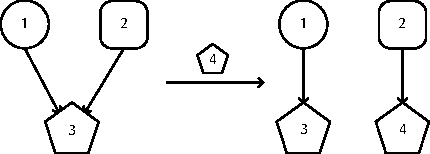
\includegraphics[width=\maxwidth{\textwidth}]{../img/react-references.pdf}
  \caption{Ukázka problému immutability a referencí}
  \label{fig:immutability-references}
\end{figure}

Problém s referencemi lze vyřešit tím, že každá odkazovaná třída v modelu bude mít datovou složku \texttt{id}, která bude instance unikátně identifikovat.
Potom instance jiných tříd budou referovat pomocí těchto složek.
Podobně je tomu například v relačních databázích.
Nevýhodou je, že může dojít ke dvěma nevalidním stavům: instance s daným \texttt{id} už neexistuje (např. byla smazána), nebo jich existuje více (došlo chybně k duplikaci objektu bez změny \texttt{id}).
Systém by se měl postarat o to, aby k tomu nedošlo.
Bohužel jsme se tímto připravili také o některé výhody, které v JavaScriptu poskytuje \acrfull{gc}.
Mezi objekty referujeme způsobem, o kterém \acrshort{gc} nemůže vědět.

Teď když známe všechny restrikce na náš model, můžeme ho začít navrhovat.
Stejně jako pro konceptuální model k tomu použijeme \acrshort{uml} třídy s komentářem v textu.
Některé výše zmíněné povinné datové složky a atributy budeme v modelu považovat za implicitní.

Nebudeme popisovat úplně celý datový model kvůli jeho rozsahu.
Některé záležitosti, které se týkají pouze zobrazování nebo nejsou důležité ve více částech aplikace, vynecháme.

\begin{figure}[!htb]
  \centering
  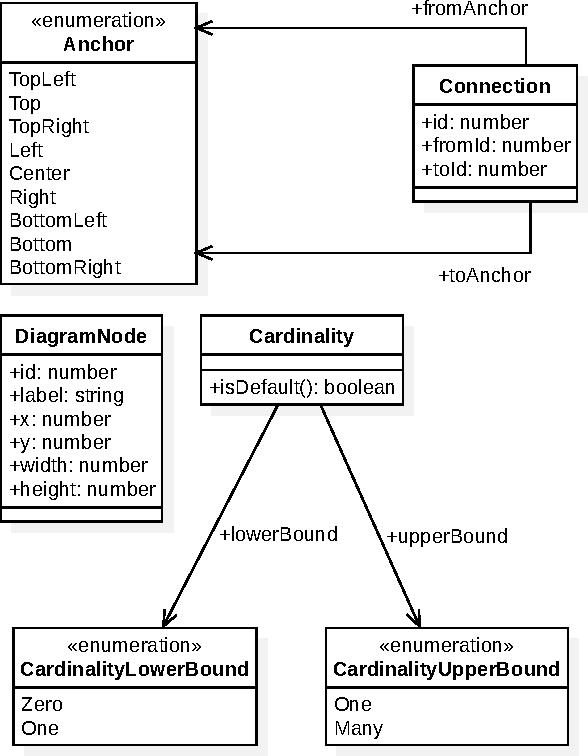
\includegraphics[width=\maxwidth{\textwidth}]{../img/diagrams/diagram-class-diagram.pdf}
  \caption{Diagram tříd -- diagram}
  \label{fig:diagram-class-diagram}
  \mcomment{Mohu zde odstranit atributy třídy DiagramNode? DiagramNode už byl popsán v předchozím diagramu, zde ho pouze využívám pro inheritanci.}
\end{figure}

Na Obrázku~\ref{fig:diagram-class-diagram} je diagram tříd popisující základní obecné konstrukty, které se týkají všech diagramů v systému.
Třída \texttt{Cardinality} obsahuje mj. operaci \texttt{isDefault}, která říká, zda se jedná o výchozí kardinalitu (námi definovanou jako \oneone).
V jazyce TypeScript, resp. JavaScript, nelze přetěžovat operátory, všechny operace musí být metody v dané třídě.
Dále v nich neexistuje koncept hodnotového porovnání instancí tříd, resp. porovnání objektů.
Pokud se porovnávají instance operátorem \texttt{==}, porovnávají se reference.

Z těchto důvodů nelze kardinalitu porovnat s jinou instancí bez přítomnosti odpovídající metody.
V našem případě je pouze potřeba zjistit, zda se jedná o výchozí kardinalitu, a proto definujeme odpovídající operaci.

Třída \texttt{Anchor} (kotva) se týká pouze zobrazení.
Říká, z a do které oblasti elementu diagramu vede odpovídající spojení.
Každý element diagramu si sám definuje a vypočítá těchto 9 kotev, které by se měly nacházet po jeho obvodu.
Tyto kotvy jsou relativní k rozměrům a umístění elementu, a proto je musí vždy přepočítat.

Kvůli restrikci o více referencích má třída \texttt{DiagramNode} své \texttt{id}.
Toto bude běžné u většiny tříd, které reprezentují elementy diagramů.

\begin{figure}[!htb]
  \centering
  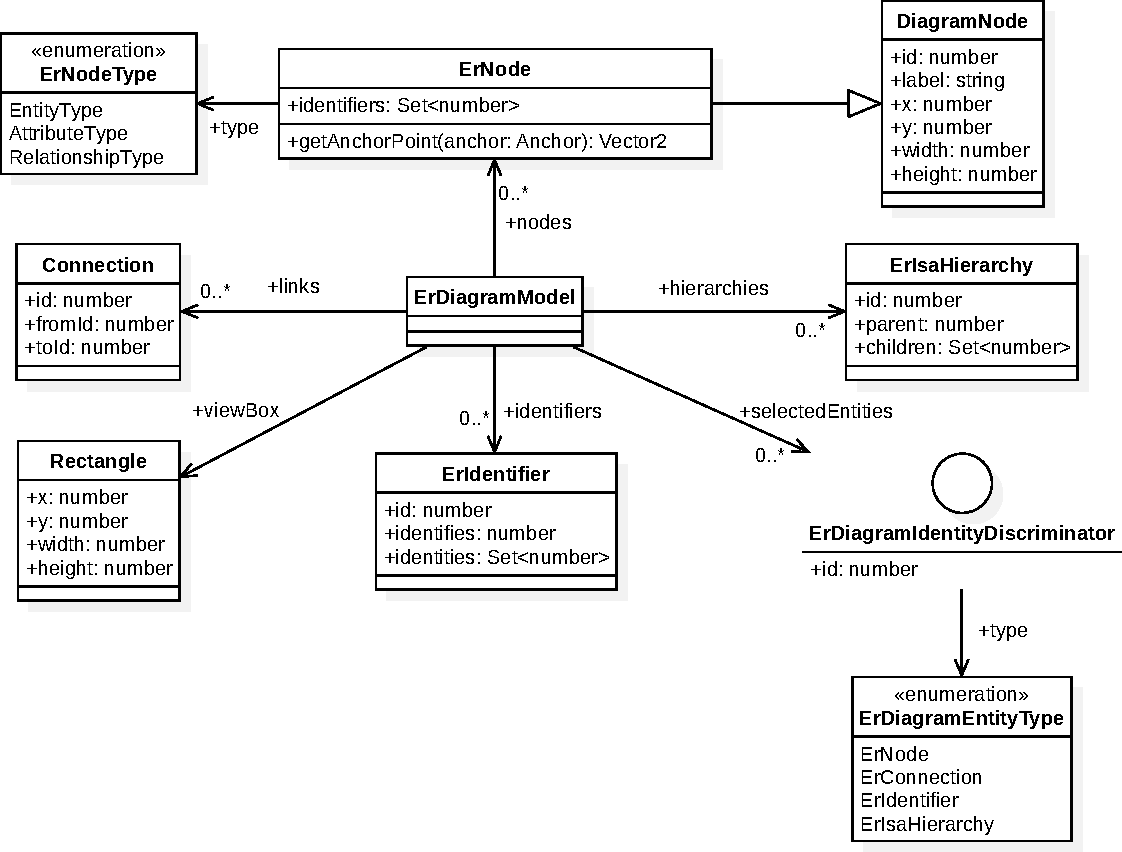
\includegraphics[width=\maxwidth{\textwidth}]{../img/diagrams/er-class-diagram.pdf}
  \caption{Diagram tříd -- \acrshort{er}}
  \label{fig:er-class-diagram}
\end{figure}

Na Obrázku~\ref{fig:er-class-diagram} je diagram tříd, které se týkají \acrshort{er} diagramu.

Hlavní třída \texttt{ErDiagramModel} je majitel svých \texttt{ErNode}, \texttt{Connection}, \texttt{ErIdentifier} a \texttt{ErIsaHierarchy}.
Pro zobrazování a uživatelskou interakci drží také interface \texttt{ErDiagramIdentityDiscriminator}, který obaluje \texttt{id} uživatelem právě vybraných elementů diagramu.
Tento obal navíc obsahuje typový diskriminátor \texttt{type}, jenž vyjadřuje, o jaký druh elementu se jedná.
Tato typová diskriminace je důležitá, aby systém věděl, kde má daný element s daným \texttt{id} hledat, zdali mezi \texttt{nodes}, \texttt{links}, \texttt{identifiers}, nebo \texttt{hierarchies}.

Podobně je určen typ \texttt{ErNode}, který pro element diagramu říká, jak se má zobrazovat.
V \acrshort{er} jsme definoval tři hlavní elementy -- entitní typ, vztahový typ a atribut.
Mohli jsme tyto elementy modelovat jako jednotlivé třídy, ale tento přístup je vhodnější, protože rozdíl mezi nimi je pouze ve vizualizaci.
Také se tímto způsobem v TypeScriptu jednodušeji pozná, s jaký typ má aktuálně držená instance \texttt{ErNode}.
V reakci na to lze jednodušeji implementovat v systému rozličnou logiku týkající se pouze jednotlivých typů elementů.

V diagramu používáme množinový typ \texttt{Set}, který je v JavaScriptu zabudovaný.
Jednodušeji se pak pracuje s odpovídajícími datovými složkami, kde nezáleží na pořadí a duplicitách.
Atributy \texttt{children} a \texttt{identities}, které tento typ mají, mají teoreticky kardinalitu \onemany{}.
V ISA hierarchii musí být alespoň jedno dítě a v identifikátoru alespoň jedna identita.

U třídy \texttt{ErIdentifier} bylo nutné názvem rozlišit jednotlivé datové složky.
Pojmenování může být matoucí, takže ho zde popíšeme.
Identifikátor (identifier) se skládá z jednoho entitního typu, jehož tímto identifikuje (identifies).
Součástí identifikátoru jsou pak jednotlivé elementy, ze kterých se identifikátor skládá.
Říkáme jim identity (identities).

Pro správné zobrazení diagramu má třída \texttt{ErDiagramModel} také datovou složku \texttt{viewBox}.
Ta vyjadřuje, na jakou část diagramu se má plátno zaměřit.
Jedná se o obdélník, který svou pozicí vyjadřuje přesun plátna a svou šířkou a výškou vyjadřuje přiblížení.
Třída \texttt{Rectangle} je obecná, a používá se proto i v jiných částech systému, kde je potřeba pracovat s obdélníky.


\begin{figure}[!htb]
  \centering
  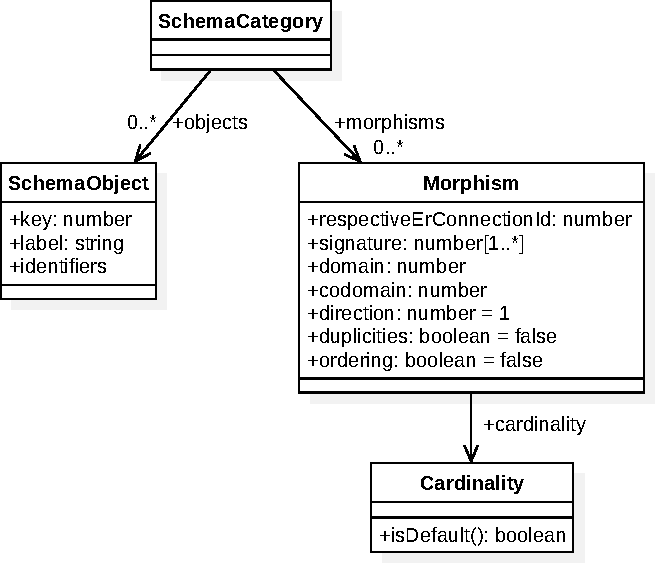
\includegraphics[width=\maxwidth{\textwidth}]{../img/diagrams/schemcat-class-diagram.pdf}
  \caption{Diagram tříd -- schematická kategorie}
  \label{fig:schemcat-class-diagram}
\end{figure}

Digram tříd, které se týkají schematické kategorie je na Obrázku~\ref{fig:schemcat-class-diagram}.
Význam většiny obsahu tohoto diagramu je evidentní.
Upozorníme pouze na atribut \texttt{respectiveErConnectionId}.

Tento atribut vyjadřuje \texttt{id} \acrshort{er} spojení, z kterého daný morfismus vznikl.
Tato informace je užitečná pro aktualizaci morfismu v návaznosti na úpravu \acrshort{er} diagramu.
Také naopak lze při úpravě schematické kategorie některé změny převést zpět do \acrshort{er}.

Objekty schematické kategorie, které vznikly převodem z \acrshort{er} budou mít stejnou hodnotu \texttt{key} jako \texttt{id} odpovídajícího objektu.
Tím zaručíme stejnou svázanost diagramů jako tomu je u morfismů.

\begin{figure}[!htb]
  \centering
  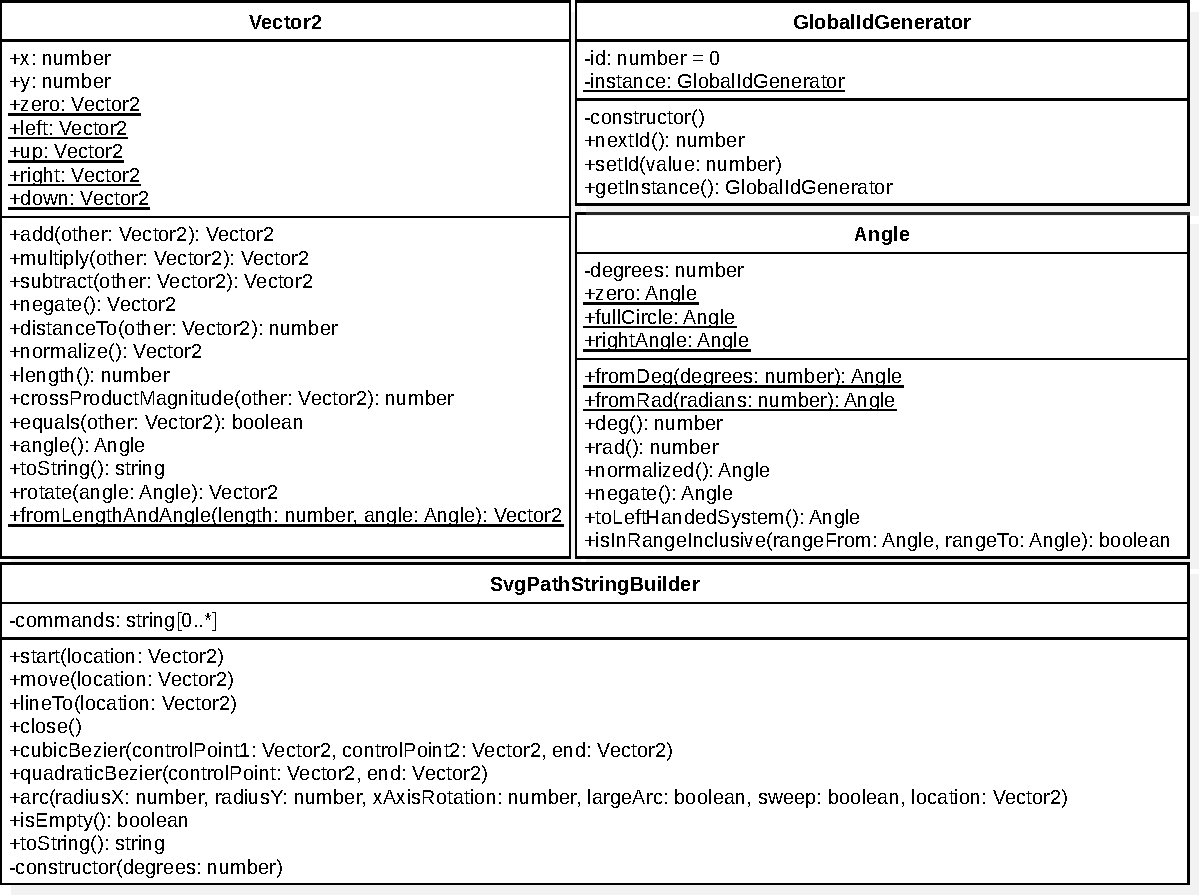
\includegraphics[width=\maxwidth{\textwidth}]{../img/diagrams/utils-class-diagram.pdf}
  \caption{Diagram tříd -- vybrané další třídy}
  \label{fig:utils-class-diagram}
\end{figure}

Další vybrané třídy, které ale nesouvisí přímo s diagramy, jsou na Obrázku~\ref{fig:utils-class-diagram}.
Pro práci s 2D geometrií budeme potřebovat třídy \texttt{Vector2} a \texttt{Angle}.

Třída \texttt{Vector2} reprezentuje dvourozměrný vektor s vhodnými operacemi včetně sčítání a odčítání s jinými vektory, násobení skalárem a negace (unární minus).
Další operace jsou vidět na Obrázku~\ref{fig:utils-class-diagram} a jejich význam by měl být evidentní.
Třída poskytuje také běžně používané vektory jako statické atributy.
Operace, které pracují s úhly, používají k jejich reprezentaci třídu \texttt{Angle}.

Třída \texttt{Angle} reprezentuje úhly nezávisle na jejich jednotkách.
Je to vhodnější, než používat pouze pomocné metody, které by převáděly stupně na radiány a naopak.
Interně je úhel reprezentován ve stupních, protože při počítání s radiány by kvůli menším číslům mohlo docházet ke ztrátě přesnosti.

Metoda \texttt{normalized} převede úhel do rozsahu $[0°, 360°)$, resp. $[0, 2\pi)$.
To jak pro negativní, tak pro pozitivní úhly mimo tyto rozsahy.

\begin{figure}[!htb]
  \centering
  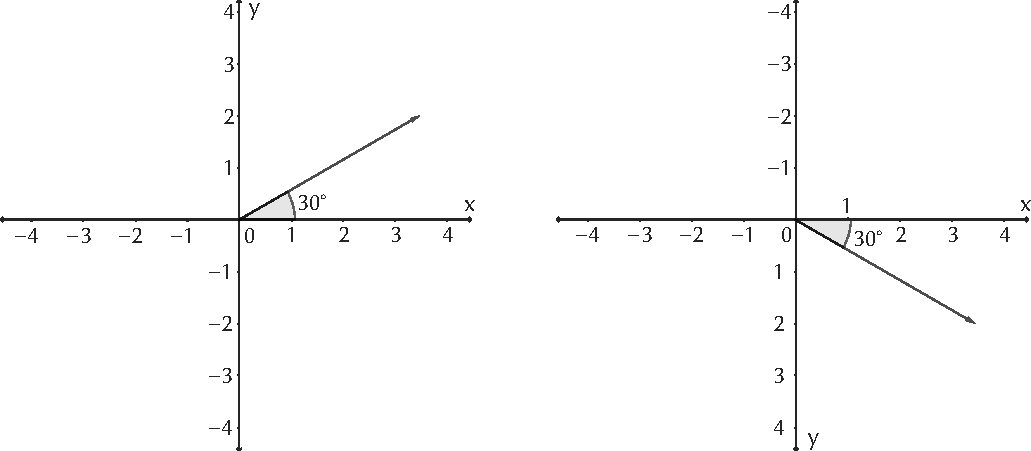
\includegraphics[width=\maxwidth{\textwidth}]{../img/cartesian-systems.pdf}
  \caption[Pravotočivá a levotočivá kartézská soustava souřadnic]{Pravotočivá (vlevo) a levotočivá (vpravo) kartézská soustava souřadnic}
  \label{fig:cartesian-systems}
\end{figure}

Na Obrázku~\ref{fig:cartesian-systems} jsou znázorněny dva typy kartézské soustavy souřadnic -- pravotočivá a levotočivá.
V matematice a geometrii je nejběžnější pravotočivá soustava souřadnic, nicméně \acrshort{svg} používá levotočivou (angl.~left-handed), jak je tomu běžné u počítačové grafiky.
Pro převod úhlu z běžně uvažovaného pravotočivého do levotočivého \acrshort{svg} úhlu slouží právě metoda \texttt{toLeftHandedSystem}.
Ta přijde vhod při rotování vektorů, či celých \acrshort{svg} konstruktů.

Třída \texttt{GlobalIdGenerator} slouží jako generátor identifikátorů a klíčů pro naše objekty.
Zajišťuje, že vždy vrátí unikátní číslo jako nový identifikátor.
Jednoduchá implementace je začít s číslem 0 a každé další zvětšit o 1.
Tato třída je singleton, jeden z objektově orientovaných designových vzorů uvedený Gammou a kol. (také známých jako \enquote{Gang of Four})~\cite[s.~144]{gamma_designpatterns_1995}.
Tím může existovat nejvýše jedna její instance v běžícím systému.

Třída \texttt{SvgPathStringBuilder} konstruuje \acrshort{svg} path data atribut \cite[\S~9.3]{brinza_svg_2018}.
Obsahuje mnoho dalších metod kromě těch, které lze vidět na Obrázku~\ref{fig:utils-class-diagram}, například pro každý příkaz lze pozice (location) specifikovat i relativně k předchozí pozici (místo absolutně).
Třída odpovídá vzoru builder~\cite[s.~110]{gamma_designpatterns_1995}.
Užívání této třídy odpovídá vypisování \enquote{příkazů} pro path data atribut.
Užitečnost této třídy spočívá v přehlednosti -- je lepší používat její metody s deskriptivním názvem místo path data příkazů, které mají formu jednoho písmene a argumentů.

\section{Scénáře}

Případy užití definují funkcionalitu systému a reprezentují se diagramem případů užití (use case diagram).
Každý případ užití popisuje jeden způsob, jak lze systém použít.
Uživatelé systému (lidé, stroje, nebo jiné systémy) jsou v diagramu reprezentováni tzv. herci (actors).
Model tak popisuje způsoby, kterými lze systém použít jeho okolím a jaké služby systém nabízí.~\cite[s.~65]{overgaard_usecases_2005}

Případy užití nebudeme popisovat všechny, kvůli stručnosti.
Dále některé případy užití jsou si velmi podobné, například export do \acrshort{svg} je téměř stejný jako export do \acrshort{png}, akorát se u \acrshort{svg} nevolí barva pozadí.
Zvolíme tedy případy užití, které nějak modelové nebo zásadní.

\begin{figure}[!htb]
  \centering
  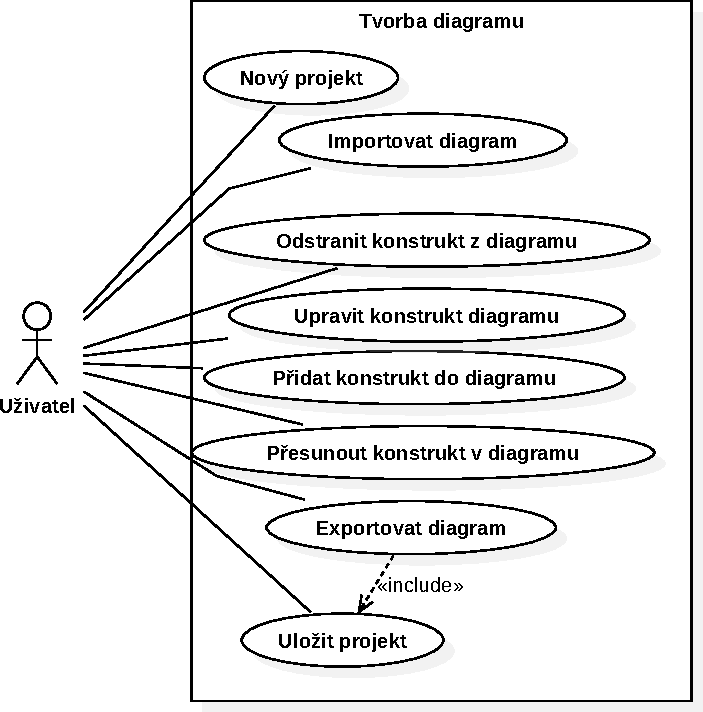
\includegraphics[width=\maxwidth{0.7\textwidth}]{../img/diagrams/use-case-diagram.pdf}
  \caption{Diagram případů užití}
  \label{fig:use-case-diagram}
\end{figure}

\newcommand{\ucsub}[1]{\textbf{#1}}
\newcommand{\uc}[1]{\subsection*{#1}}
\def\ucstart{\ucsub{Počáteční stav}\\\indent}
\def\ucnormal{\ucsub{Běžný průběh}}
\def\ucerrors{\ucsub{Možné chyby}}
\def\ucend{\ucsub{Stav systému po dokončení}\\\indent}

\uc{Přidání entitního typu do \acrshort{er} diagramu}
\ucstart{}
V systému je rozdělaný projekt.
\acrshort{er} diagram lze editovat.

\ucnormal{}
\begin{enumerate}
  \item Uživatel přetáhne myší konstrukt \enquote{entitní typ} z panelu konstruktů do \acrshort{er} diagramu.
  \item V diagramu je vytvořen nový entitní typ s výchozím názvem.
  \item Uživatel zvolí právě vytvořený entitní typ myší.
  \item V panelu \enquote{Control Panel} upraví vlastnost entitního typu \enquote{label}.
  \item Název entitního typu se změní na uživatelem definovaný.
\end{enumerate}

\ucend{}
V diagramu je nový entitní typ, který má uživatelem definovaný název.
Změna se projeví i ve schematické kategorii, respektive ve \acrshort{vsk}.

\uc{Přidání atributu k entitnímu typu v \acrshort{er} diagramu}
\ucstart{}
V \acrshort{er} diagramu je entitní typ. Diagram lze editovat.

\ucnormal{}
\begin{enumerate}
  \item Uživatel pravým tlačítkem myši klikne na entitní typ.
  \item Otevře se kontextové menu.
  \item Uživatel zvolí položku \enquote{Add attribute type}.
  \item Do \acrshort{er} diagramu je přidán nový atribut, který je spojen s entitním typem.
  \item Uživatel zvolí právě vytvořený atribut myší.
  \item V ovládacím panelu upraví vlastnost \enquote{label}.
  \item Název atributu je nastaven na právě uživatelem definovaný.
  \item Uživatel případně zvolí spojení mezi entitním typem a atributem myší.
  \item V ovládacím panelu zvolí kardinalitu ze čtyř předdefinovaných možností.
  \item Tato kardinalita je pro spojení nastavena.
\end{enumerate}

\ucend{}
V modelu systému je uložen nový atribut entitního typu, který má daný název a kardinalitu.
Změna se projeví i ve schematické kategorii, resp.~ve \acrshort{vsk}.

\uc{Přidání spojení mezi dva \acrshort{er} elementy diagramu}
\ucstart{}
V \acrshort{er} diagramu dva existující elementy.

\ucnormal{}
\begin{enumerate}
  \item Uživatel zvolí první element levým tlačítkem myši.
  \item Uživatel klikne na druhý element pravým tlačítkem myši.
  \item Zobrazí se kontextové menu.
  \item Uživatel zvolí položku \enquote{New connection}.
  \item Mezi elementy se vloží spojení.
\end{enumerate}

\ucerrors{}
\begin{itemize}
  \item Elementy mohou být nekompatibilní -- např. dva vztahové typy, dva entitní typy.
\end{itemize}

\ucend{}
V modelu i v zobrazeném diagramu bude mezi elementy nové spojení.
\uc{Přidání vztahového typu do \acrshort{er} diagramu}
\ucstart{}
V diagramu je entitní typ nebo více entitních typů, které se budou účastnit vztahového typu.
Případně je lze vytvořit i v průběhu toho případu užití.
Změna se projeví i ve schematické kategorii, resp.~ve \acrshort{vsk}.

\ucnormal{}
\begin{enumerate}
  \item Uživatel z panelu s konstrukty myší přetáhne vztahový typ do \acrshort{er} diagramu.
  \item V \acrshort{er} diagramu se objeví nový vztahový typ.
  \item Uživatel v ovládacím panelu změní název vztahového typu.
  \item Uživatel spojí entitní typ se vztahovým typem podle už popsaného případu užití spojování elementů. Tím přidá účastníka vztahového typu.
  \item To zopakuje s dalšími účastníky (ne nutně jinými).
\end{enumerate}

\ucend{}
V systému je nyní nový vztahový typ s účastníky. To se projeví i ve schematické kategorii, resp.~\acrshort{vsk}.

\uc{Export libovolného diagramu do \acrshort{png}}
\ucstart{}
V systému je rozdělaný projekt.

\ucnormal{}
\begin{enumerate}
  \item Uživatel zvolí položku \menu{File > Export as > PNG} v hlavním menu aplikace.
  \item Otevře se dialog s možnostmi exportu s výběrem diagramu k exportu. Výchozí zvolený diagram bude ten, ve kterém naposledy uživatel pracoval.
  \item V dialogu dále uživatel zvolí, jestli chce do \acrshort{png} souboru zahrnout i serializovanou verzi projektu, aby šel později \acrshort{png} soubor otevřít v aplikaci.
  \item Uživatel v dialogu dále zvolí, jestli má \acrshort{png} mít barvu pozadí, případně jakou. Výchozí nastavení je \acrshort{png} bez pozadí, tedy transparentní.
  \item Uživatel potvrdí dialog.
  \item V prohlížeči uživatele se \enquote{stáhne} exportovaný \acrshort{png} soubor, který má název odpovídající názvu projektu.
\end{enumerate}

\ucerrors{}
\begin{itemize}
  \item V zařízení uživatele není dostatek persistentní paměti na uložení obrázku. O zachycení a obstarání této chyby se stará webový prohlížeč uživatele.
  \item Uživatel zruší dialog místo potvrzení. V takovém případě se nic dalšího nestane (nedojde k exportu).
\end{itemize}

\ucend{}
V uživatelské složce nastavené ve webovém prohlížeči na uložení stahovaných souborů bude uložen \acrshort{png} soubor s rasterizovaným diagramem.
